\documentclass{article}
\usepackage[utf8]{inputenc}
\usepackage[T1]{fontenc}
\usepackage{geometry}
\usepackage{graphicx}

\geometry{margin=0.5in}

\begin{document}
\section*{Task}
You need to modify the program that continuously generates a sinusoidal waveform. The modification involves introducing a regulated limit on the output waveform.

\subsection*{\underline{Task conditions}}
\begin{enumerate}
    \item the function to adjust the frequency of the output waveform must be retained
    \item \textit{a limit} must be introduced on the value of the sinusoidal output waveform
    \begin{enumerate}
        \item the limit is symmetrical with respect to the center value of the sinusoidal waveform
        \item the limit value is adjusted using two buttons – up/down
        \item changing the limit value must not affect the frequency
    \end{enumerate}
    \item the program is supposed to be implemented using interrupts (\underline{without using the resources of the main program})
\end{enumerate}

\begin{center}
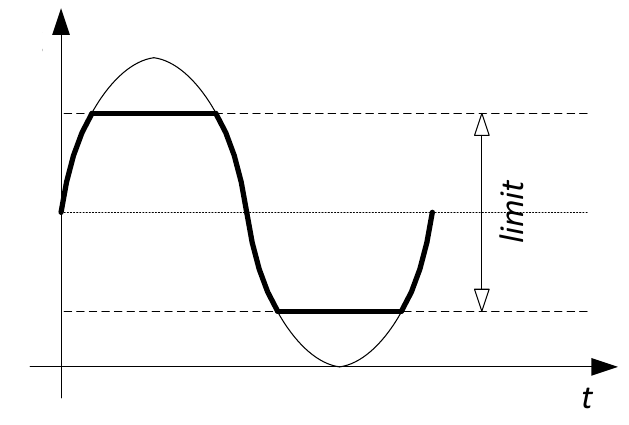
\includegraphics[width=0.5\textwidth]{../img/DAC_sinus_limit.png}
\end{center}
\end{document}